\paragraph{QuizziPedia::Front-End::Directives::OneQuestionDirective}

\label{QuizziPedia::Front-End::Directives::OneQuestionDirective}

\begin{figure}[ht]
	\centering
	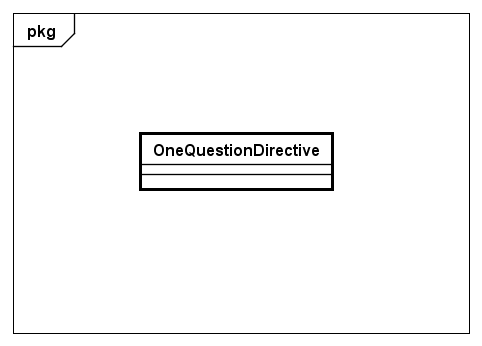
\includegraphics[scale=0.80,keepaspectratio]{UML/Classi/Front-End/QuizziPedia_Front-end_Directives_OneQuestionDirective.png}
	\caption{QuizziPedia::Front-End::Directives::OneQuestionDirective}
\end{figure} 
\FloatBarrier

\begin{itemize}
	\item \textbf{Descrizione}: rappresenta il componente grafico che visualizza all'utente l'anteprima della domanda che ha creato. Eseguendo l'azione di click sul pulsante di modifica sarà possibile modificare tale domanda. All'interno di \texttt{QuestionsManagementsView} verranno stampati a video tanti componenti quanti presenti nello \texttt{\$scope} isolato ad esso associato;
	\item \textbf{Utilizzo}: viene utilizzato per permettere all'utente di visualizzare le domande che ha creato;
	\item \textbf{Relazioni con altre classi}: 
	\begin{itemize}
		\item \textit{IN} \texttt{QuestionsManagementView}: view contenente l'elenco delle domande create;
		\item \textit{IN} \texttt{LangModel}: rappresenta il modello delle informazioni per la giusta traduzione dell'applicazione. 
	\end{itemize}
	\item \textbf{Attributi}: 
	\begin{itemize}
		\item \texttt{+ data: Object} \\ Oggetto contenete le informazioni da mostrare nell'anteprima della domanda;
		\item \texttt{+ modifyButtonOneQuestion: String} \\ Attributo che viene utilizzato per visualizzare la giusta traduzione della \textit{label\ped{G}} per il bottone di modifica della domanda, in italiano o in inglese;
		\item \texttt{+ restrict: String} \\ Stringa che permette di definire le modalità di inserimento della direttiva all'interno della pagina;
		\item \texttt{+ scope: Scope}: oggetto scope interno della direttiva, contiene le funzionalità per gestire i dati presenti all'interno;
		\item \texttt{+ templateUrl: String} \\ Stringa contenente il percorso del file \textit{HTML\ped{G}} che contiene la direttive.
	\end{itemize}
\end{itemize}